

The following results are based on simulations of the model with parameter values given in
\autoref{tab:parameter}. {\bf (Erich do you remember how we chose these numbers?)}  The grid size was 101 patches by 101 patches.
The standard error was calculated by dividing the sample standard deviation by the square root of
the total number of samples.   The standard errors were all less than 1\% on average, so will not be
shown due to the small size.

\begin{table}
  \begin{tabular}{|l|l|l|l|}
    \hline
    % after \\: \hline or \cline{col1-col2} \cline{col3-col4} ...
    Parameter Description & Symbol & Value &  \\ \hline  \label{parameter}
    Total number of animals & b & 1,000 & fixed  \\ \hline
    Maximum time & $t_{max}$ & 1,200 seconds & fixed \\ \hline
    Fraction of blooms at one time & a & 0.2 & fixed \\ \hline
    Maximum fraction of available flowers & $\eta$ & 0.75 & fixed \\ \hline
    Search radius & r & 1.0 & fixed \\ \hline
    Number of flowers per plant & $\phi$ & 100 & fixed \\ \hline
    Probability of pollination   & $\rho$ & 0.4286 & calculated \\ \hline
    Number of plants & n & 1000 & fixed \\ \hline
    Time spent at each plant & $t_{plant}$ & 100 seconds & fixed \\ \hline
  \end{tabular}
  \caption{Parameter Values}
  \label{tab:parameter}
\end{table}


%The distance animals travel during a foraging trip is important factor for their
%survivability.  In order for an animal to survive it must find enough food foraging without losing
%too much energy.  In this study the density of plants is varied, which can directly affect the
%amount of foraging the animals will be able to achieve in a set amount of time.  The higher the
%density the greater the potential for the animal to forage.  The maximum angle is also varied.  The
%relationship of this angle with respect to foraging is a more complicated one.  In terms of
%foraging, a very small maximum turning angle may not result in successful foraging due to the paths
%are too linear.  On the other hand, a maximum turning angle which is too large can result in
%searching patterns that repetitively cover the same area over and over again.

%{\emph{Average Path Distance}}
\begin{figure}
  \begin{center}
  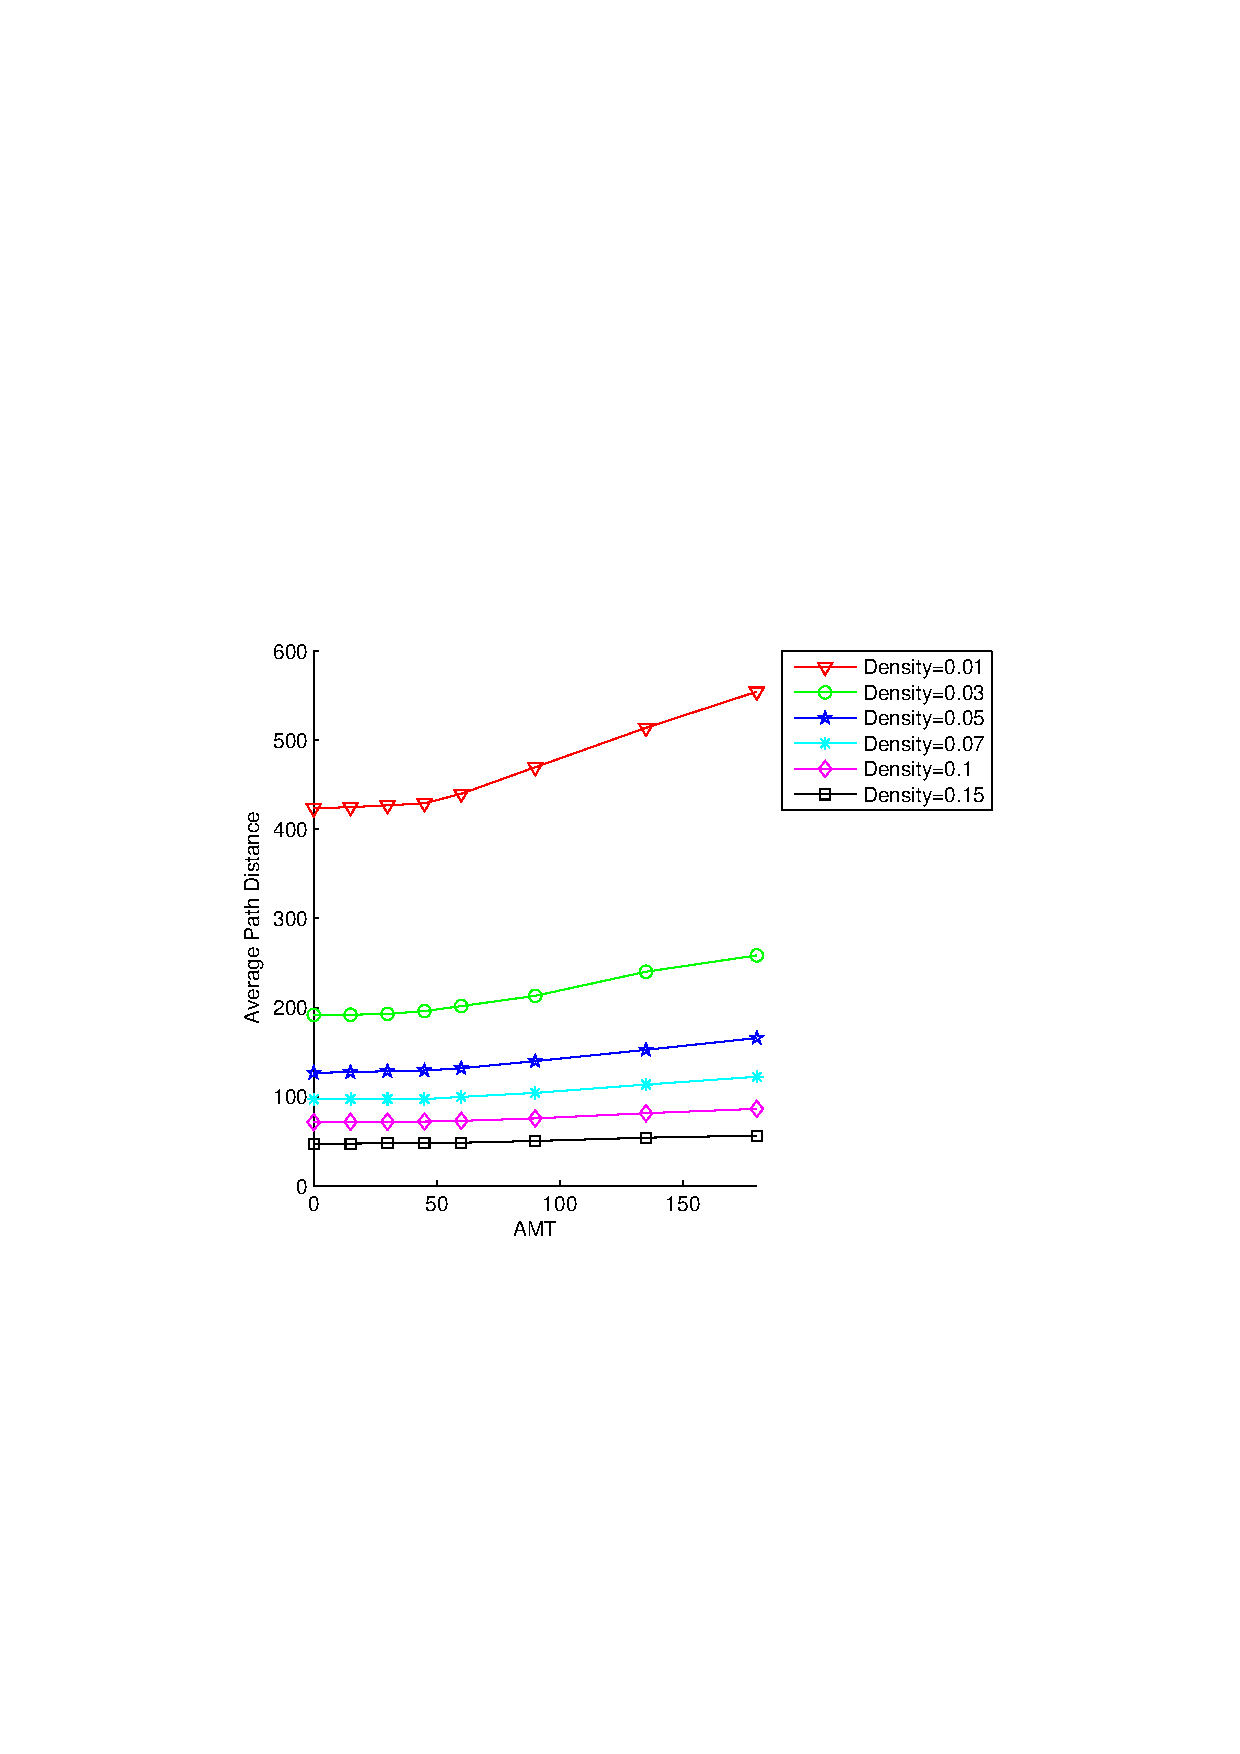
\includegraphics[scale=0.5, trim=0 240 50 300]{PathVsAMT.pdf}
  \end{center}
  \caption{\small Average Path Distance vs. Turning Angle for Various Plant Densities}
  \label{AvgPathN}
\end{figure}

In \autoref{AvgPathN} the average distance traveled for each animal decreases with increasing
density due to higher foraging success.  In this situation the animals will spend more time on
plants since they can find plants more readily and thus reach their maximum searching time more quickly.  The maximum turning angle does not have a large
effect on on the  average distance in general, though there is a modest effect at low plant densities
where the larger values increase the average distance due to less success at foraging.

On the other hand, the average maximum distance traveled by animals, see \autoref{AvgMaxDBees}, is affected by both
the turning angle and plant density. As with the average path distance, the maximum distance
decreases with higher density for the same reason that this decreases the overall travel time for the
animals since they spend more time on plants.  In
this case due to the movement patterns the maximum turning angle has a large effect on maximum distance traveled especially
at lower densities.  As the maximum angle decreases the animals are moving in a more highly correlated random walk and are more likely to travel directly
away from their starting points increasing the maximum distance traveled.

In particular at high density for a moderately correlated random walk $(AMT=90^{\circ})$ there is an increase of over 30\% for the maximum distance over the purely random walk, and for a highly correlated random walk $(AMT=45^{\circ})$ there is an increase of 67\%.  At lower densities this is more pronounced.  There is an increase in the maximum distance traveled by 62\% and 160\% over the purely random walk by a moderately and highly correlated random walks, respectively. These differences can have important consequences on the overall genetic diversity for the plants, and shows that biotic dispersal has a greater potential for long range pollination over abiotic dispersal.  

%\subsubsection*{\emph{Average Maximum Distance}}
\begin{figure}
  \begin{center}
  \includegraphics[scale=0.5, trim=50 240 50 300]{MaxDVsAMT.pdf}
  \end{center}
  \caption{\small Average Maximum Distance vs. Turning Angle for Various Plant Densities}
  \label{AvgMaxDBees}
\end{figure}

We see this potential in \autoref{AvgDist} where, like the average maximum distance, the average pollination distance increases with stronger correlation and at lower density.  At high densities the effects of correlation are smaller.  This is due to the fact that as pollinators visit more plants they leave each plant in a random direction which consequently has them to behave more like a purely random walk.  It is also the case as with the average maximum distance, as the
maximum angle decreases and the correlation strengthens, the animal is likely to travel farther from its initial position which
allows for longer pollination distances.

At low densities there in an increase in the average pollination distance of 36\% and 96\% over a purely random walk for a moderately and highly correlated random walk, respectively.  At high density the increases are 29\% and 65\%, respectively.  These increases will have significant impact on the overall gene flow of the plant species.

%\subsubsection*{\emph{Average Pollination Distance}}
\begin{figure}
  \begin{center}
  \includegraphics[scale=0.5, trim=50 240 50 300]{PollenDVsAMT.pdf}
  \end{center}
  \caption{\small Average Pollination Distance vs. Turning Angle for Various Plant Densities}
  \label{AvgDist}
\end{figure}


These increases are also observed for the maximum pollination distance.  For low plant densities the average maximum pollination distance increases by 53\% for moderately correlated random walks over purely random walks, and 148\% for highly correlated random walks.
 Additionally, for high plant
densities these increases are 44\% and 96\% for moderately and highly correlated random walks over purely random walks, respectively.  Since these are average values there is clearly a potential for much greater range of pollen dispersal and genetic variation with biotic dispersal over abiotic dispersal.

%\subsubsection*{\emph{Average Maximum Pollination Distance}}
\begin{figure}
  \begin{center}
  \includegraphics[scale=0.5, trim=50 240 50 300]{MaxPollenVsAMT.pdf}
  \end{center}
  \caption{\small Average Maximum Pollination Distance vs. Turning Angle for Various Plant Densities}
  \label{AvgMaxDTreesN}
\end{figure}

%The average maximum pollination distance has a much more complicated relationship with density and
%maximum turning angle.  The average maximum pollination distance
%decreases as maximum turning angle increases from $0^{\circ}$ to $180^{\circ}$ across all densities.
%This is due to animals covering a shorter distance for higher turning angles, and therefore the
%plants that are visited will be closer together on average.

%Additionally, we see that the average maximum pollination distance for a purely random
%diffusion process is marketably lower than those for correlated random walks. Thus, abiotic dispersal will result in an average maximum pollination distance %that is
%less than the average maximum pollination distance for biotic dispersal. Thus, one might
%expect that wind dispersal of pollen results in a smaller area extent of gene flow as compared to
%animal mediated gene flow.

Plant density affects the maximum pollination distance in a more complex fashion.  The higher the
density the more gradual the decrease is in the maximum pollination distance as the maximum turning
angle increases.  Whereas at lower densities this decrease is much larger.  This is due to
the fact at lower densities pollination occurs less frequently with a larger variability of
maximum pollination distances.

%\subsubsection*{\emph{Average Weighted Diversity of Fathers}}
\begin{figure}
  \begin{center}
  \includegraphics[scale=0.5, trim=0 240 50 300]{WDFvsAMT.pdf}
%  \includegraphics[width=1.0\textwidth,height=0.5\textheight]{WDFvsAMT.pdf}
  \end{center}
  \caption{\small Average Weighted Diversity of Fathers vs. Turning Angle for Various Plant Densities}
  \label{EFathers}
\end{figure}

In general there is a small decrease in the average weighted diversity of fathers as the maximum
turning angle increases, see \autoref{EFathers}. With higher maximum turning angles the search
patterns tend to be more circular lowering the overall diversity that a plant will see since pollinators will visit the same plants more frequently.  On the
other hand, by increasing the density, plants will see an increase in diversity due to the larger
amount of plants near by.  This increase lessens at higher densities due to the limited foraging
time of the pollinators.
